\chapter{Interconnect and Memory Management}
\label{chap:interconnect}

This chapter discusses how the data is transported 
from the main memory to an accelerator and vice versa. 
Essentially, this covers the communication protocol 
and its underlying physical interconnect, 
as well as their impact on system performance 
and software complexity.

The choices made in hardware architecture is 
a trade-off between silicon area, clock speed and flexibility. 
The latter takes the form of restrictions on memory view from the FPGA side, 
which necessitates proper software support 
for the memory allocator and acclerator scheduler.

The software framework, more precisely the kernel module,
is flexible enough to support a wide diversity of system configurations. 
To demonstrate this, there have been implemented two hardware designs: 
The first is geared to accelerator performance featuring wider interconnect that 
allows greater data processing parallellization,
homogeniety of reconfigurable partitions that allows freedom of accelerator placement, 
and full memory view on the accelerator side, maximizing the scheduler's decision options.
The second once is geared to high accelerator core count 
that sacrifices per-core performance and flexibility.
It uses narrower and simpler interconnect that lacks intermediate buffering. 
More importantly, it segments the memory view, 
imposing restrictions on accelerator placement. 
Finally, it features two types of reconfigurable partitions,
further complicating scheduler.

Provided that a proper hardware description 
in the form of a Device Tree\cite{devicetree}, 
the kernel module will detect the hardware 
configuration and execute the requested task list 
without the need of source code modification or even a recompilation.

\section{The Communication Protocol}

In order for two (or more) entities to exchange data, 
there must be a well-defined protocol.
With the growth of FPGA ecosystem, a need for a common 
and widespread communication protocol arose,
in order to replace custom solutions that deemed 
too inflexible for bigger designs comprising IP
from different projects teams and different companies.
The ARM's proposal is the \gls{amba}\cite{amba} 
which as the name suggests was initially deployed 
for microcontroller use but later expanded to SoCs,
has gained momentum due to ARM's dominance in smartphone market. 
Since all modern FPGA-SoCs from Xilinx use ARM cores, 
it became a natural choice for the company. 
Earlier products of Xilinx, like Virtex-II Pro which
featured a PowerPC core, used IBM's CoreConnect bus architecture. 
The other big contender is the free and open source ``Wishbone Protocol'', 
which, not unexpectedly, is the favorite of 
``OpenCores'' open-source hardware community.

The Zynq 7000 platform, as well as the newer Zynq UltraScale+, 
the two platforms that are targeted by this work,
both feature ARM cores and are designed around the \gls{axi} protocol,
which is part of the \gls{amba} suite. 
Furthermore, Xilinx, in order to promote IP reuse with its IP Integrator tool
has expanded its use in its FPGAs that contain no ARM IP. 
The \gls{axi} infrastructure and several basic \gls{axi} peripherals
are offered by Xilinx in Vivado at no additional cost.
Therefore, \gls{axi} was chosen for the development of this system.

It is important to note that \gls{amba} protocols are for on-chip interconnect only.
Although they can transverse the PS-PL border,
they are never exposed outside of the chip. 
This stands true not only for Xilinx's -- or Altera's -- FPGAs, 
but also for all ARM-based microcontrollers and SoCs.

\subsection{The AMBA AXI Family}

\label{amba}
The \gls{axi} itself is essentially a group of protocols that support different topologies,
as well as feature levels that position themselves differently at the trade-off 
between performance and functionality versus silicon area.

Tha \gls{axi} family has several members, but for this system the following three were used:
\begin{itemize}
\item	\textbf{\gls{axi}}, was the initial and only member in \gls{amba} 3.0. 
	With the advent of \gls{amba} 4.0 which introduced
	the protocols mentioned below, it is now usually 
	referred as ``Full \gls{axi}'' or ``\gls{axi} Memory Mapped''.
	It connects one or more memory capable slave to the 
	address spaces of one or more masters. 
	It typically needs glue logic between the two endpoints, 
	called ``\gls{axi} Interconnect''. 
	The address must be communicated before transfer takes place, 
	which consists a performance barrier.
	To amend this, it supports \gls{burst} mode, 
	where sequential packets of data may be transferred without
	re-transmitting any addressing information. 
	It is a high performance protocol, 
	suited for exchange of large amount of data. 
	Its typical use in the FPGA world is 
	transferring data between memory resources,
 	like Block RAMs, processing system RAM, 
	external memory controllers connected to the FPGA, etc.
\item	\textbf{\gls{axi}-Lite}. Introduced with \gls{amba} 4.0, 
	the \gls{axilite} as the  name implies 
	is a reduced capability version of \gls{axi}. 
	The most notable omission is the support for \gls{burst} transfers. 
	In exchange, it offers a much lower silicon footprint. 
	It is best suited for low intensity traffic, 
	typically in configuration registers.
\item	\textbf{\gls{axi}-Stream}. Also introduced with \gls{amba} 4.0, 
	\gls{axi}-Stream is a data streaming protocol,
	which means that it has no notion of memory addressing.
	This greatly simplifies implementation and reduces wire count.
	Data flows from the one endpoint to the other, in one direction, 
	without the need of any intermediary interconnect.
	It may serve any streaming application and it allows 
	the addition of user defined out-of-band data,
	typically for synchronization, and it supports sender and receiver IDs, 
	which enables stream switching and virtual circuits.
\end{itemize}

None of these protocols supports cache coherency. 
In \gls{amba} 3.0, ARM proposed the \gls{acp}, 
an \gls{axi} slave port that connects an \gls{axi} master directly to the processor.
The coherency logic inside the processor 
will monitor the transactions and update its caches accordingly.
However, since the \gls{axi} master is not aware of the cache coherency logic, 
\gls{acp} is an \gls{IO Coherency} mechanism;
the processor caches may be coherent but the accelerator's may not.

In \gls{amba} 4.0, ARM extended the \gls{axi} protocol with \gls{ace},
\gls{axi} Coherent Extensions, which allows full coherency between
the processor and the accelerator, and \gls{ace}-Lite, 
an \glslink{IO Coherency}{IO Coherent} version. 
Finally, in latest \gls{amba} version, 5.0, ARM added \gls{chi}, 
which targets the multiprocessor's local interconnect hub.

In the data streaming model, there exists no spatial or temporal locality. 
Cached transfers are not only useless but harmful, since they will cause cache thrashing. 
Indeed, the kernel driver uses the Linux DMA Streaming API
which bypasses all processor caches by marking 
the allocated DMA'able pages as non-cacheable.
Therefore, cache coherency will not matter our discussion any further.

\subsection{The AXI Implementation}

The \gls{axi} implementation in Xilinx products consists of the hardware 
implementation in Zynq 7000 and Zynq UltraScale+ devices,
the \gls{soft-ip} protocol infrastructure offered in IP Integrator, 
and the \gls{axi} compatible IP building blocks. 
Additionally, Xilinx offers automation for creating 
custom cores with \gls{axi} interfaces.
It is worth to cover this functionality as 
part of understanding the connectivity of the system.

\subsubsection{The Zynq Hard IP}

The Zynq 7000 is built around \gls{amba} 3.0. 
The interconnect will be presented at the next section,
but it is important to mention here that 
the use of \gls{axi} of this \gls{amba} version
carries two important restrictions: 
The original specification of \gls{axi},
as is present in \gls{amba} 3.0 has a maximum \gls{burst} size of 16. 
Any \gls{axi} master residing in PL that connects to the PS through a slave port,
will have to obey this limit or use a protocol converter.
Secondly, \gls{amba} 3.0 does not support \gls{axilite} or \gls{axistream}, 
therefore all ports that connect the PL to the PS are Full \gls{axi}.

\subsubsection{The Xilinx Soft IP}
\label{sect:xilinx-ip}

At the PL front, Xilinx offers a suite of 
IP cores that manipulate the \gls{axi} traffic.
It offers cores for conversion (stream combining, 
width conversion), buffering (clock conversion,
stream pipelining, \gls{fifo} buffer) and routing 
(stream broadcasting, stream switching, \gls{axi} crossbar).
Additionally there are some higher level \gls{axi} building blocks
that automate the interconnect of \gls{axi} endpoints. 
Due to their importance, it is worth to be mentioned separately:

\begin{itemize}
\item	\textbf{AXI Stream Interconnect}. 
	This core can interface $M$ \gls{axi}-Stream masters to $N$ slaves.
	It's built around an \gls{axi}-Stream switch with appropriate
	couplers in each of its interfaces.
	The role of couplers are to perform the necessary protocol conversions and/or buffering.
	The routing may either be defined externally through 
	a configuration register or by 	the sender / receiver IDs. 
	It should be stressed that in contrast to its Full \gls{axi} counterparts, 
	it is not an essential core if only a single master is connected to a single slave.
	Its use arises on shared physical links and/or where virtual circuit switching is needed.
\item	\textbf{AXI Interconnect}. 
	The equivalent interconnect for Full \gls{axi}, that can connect $M$ masters
	to $N$ slaves communicating with either Full \gls{axi},
	both version 3.0 and 4.0, or \gls{axilite} protocol.
	The interconnect can be configured in full crossbar mode for high performance,
	or in shared access mode for low area use, issueing only one transaction at a time.
	The signals can be -- and typically are -- registered 
	and buffering can be added at either ends.
\item	\textbf{AXI SmartConnect}. 
	This core is a newer design with functionality analogous to \gls{axi} Interconnect.
	It is advertised to be highly optimized to mitigate wire delays in UltraScale+.
	The value of this core was assessed in this work along with
	the standard \gls{axi} Interconnect IP.
	It was found that it does improve clock even on Zynq 7000 series,
	but at some cost in FPGA resources. 
	In a crowded design it may complicate routing, resulting in a lower clock.
	If the design uses a slow clock for the targeted FPGA or 
	if the slaves are \gls{axilite} configuration registers,
	the older \gls{axi} Interconnect should be preferred.
\end{itemize}

As it might have become obvious, the common use of \gls{axistream} is exchange of data between the
functional units implemented in the programmable logic. Since no large memories are possible,
data flows from one unit to the other in a conitguous fashion. However, when the transfer of data
to/from the processor memory or other PL-based addressable memory is needed, the use of a DMA
controller would be typically needed. The DMA controller could be at either side, 
the fabric or the processor, and the trade-offs will be discussed at section 
\ref{sect:implementation}.
For now, let us discuss the key data transfer cores that can be implemented in the fabric.
\begin{itemize}

\item	\textbf{AXI DataMover}:
	This is the central component of all DMA controllers.
	Its role is to move data between the memory mapped and stream domain.
	Apart its Full \gls{axi} master and \gls{axi} Stream slave ports, 
	it has one \gls{axi}-S master and one slave port, 
	for status and control messages respectively.
	It can be configured as unidirectional or bidirectional.
\item	\textbf{AXI DMA}:
	The \gls{axi} DMA is essential the controller unit of DataMover. 
	An \gls{axi} DMA consists of two unidirectional or a single bidirectional
	\footnote{This configuration is not supported by Xilinx HSI for DeviceTree generation,
	which is the standard method describing hardware to the Linux kernel}
	DataMover and a controller unit that generates the command/status stream.
	That unit is configured with an \gls{axilite} interface, 
	where is presents its configuration registers.
	The core has an optional scatter-gather engine that can continuously fetch and execute
	transfer descriptors without any pause for programming.
\item	\textbf{AXI Video DMA}: 
	This core is a variation of \gls{axi} DMA specialized in video streams.
	Among other optimizations, it takes advantage of the user-defined out-of-band channel
	of \gls{axi}-Stream for frame synchronization.
\item	\textbf{Central DMA}: 
	A misnomer, its role is actually to move data between two Full \gls{axi} interfaces.
	It is implemented by a bidirectional DataMover and the control logic, with an optional
	scatter-gather engine. CDMA is apropriate when both communication endpoints are addressable
	memory s paces, eg the processor memory and an \gls{axi} BRAM controller.
\end{itemize}

%For completeness, it should be noted that communication in a Full \gls{axi} channel could be prossible
%with programmed I/O from the processor. However, no processor is able to generate data \glspl{burst}
%with load/store instructions. This would degenerate Full \gls{axi} to an \gls{axilite} link. 
%Therefore, even if we could afford to spare the processor cycles, the throughput would still suffer.
%Naturally, programmed I/O is actually the de facto access method for \gls{axilite} slaves,
%and it is typically used to program the DMA configuration registers.

\subsubsection{The User IP}

As it becomes clear, Xilinx does offer a significant amount of 
\gls{axi} infrastructure IP and \gls{axi} compatible peripherals
to support the implementation of an \gls{axi}-based system.
Still, implementation of \gls{axi} compliant custom logic is a non-trivial task to undertake.
Depending on the workflow and the designer's experience and demands,
there are five options available.

\begin{itemize}
\item	\emph{Custom Implementation}:
	In case maximum flexibility and performance is desired,
	a custom implementation is the way to go. 
	Xilinx offers \gls{axi} Verification IP that helps the designer to verify the functionality
	of an RTL design.
\item	\emph{IP Integrator}:
	Xilinx offers a ``Create and Package IP'' wizzard in its IP Integrator tool.
	The designer may define the desired \gls{axi} parameters 
	and the wizzard will generate the corresponding RTL code
	to create the \gls{axi} interface. 
	The designer can afterwards tweak the code to adapt their needs.
\item	\emph{IP Interfaces (IPIFs)}:
	IPIFs are IP cores that alleviate the burden of \gls{axi} conformance 
	from the end designer by performing the complex \gls{axi} signaling 
	themselves while offering a simple memory-like interface on the other end. 
	Xilinx provides two such cores, one for Full \gls{axi} 
	supporting \gls{burst} transactions, and one for \gls{axilite}.
	\gls{axistream} is simple enough to not necessitate such an interface.
\item	\emph{Bridges}: In case the user IP is already developed with an alternative protocol,
	it may be possible to bridged to the \gls{axi} interconnect, 
	if the added overhead can be tolerated.
	Xilinx provides only a handful of birdges, 
	mostly for within the \gls{amba} family, 
	eg for \gls{ahblite} (both slaves and masters) and for \gls{apb} (slaves only). 
	However, additional bridges may be found at OpenCores
	or in other open-source libraries. 
	In the simplest case possible, a designer may even opt for 
	the \gls{axi} \gls{gpio} core that can provide up to two 32 bit general purpose I/O lines.
\item	\emph{HLS}: If the designer uses the Vivado High-Level Synthesis workflow,
	the tool is able create \gls{axi} compliant IP using simple HLS directives. 
	This is particularily useful to implement
	the HLS-core control protocol over \gls{axilite}.
\end{itemize}

\section{The Physical Interconnect}

So far, we discussed the communication protocol and its implementation at both 
the programmable logic and the hard-ip domains.
The next logical step would be to examine the underlying physical interconnect
that supports it on the SoC-FPGAs that this work targets. 

Granted, in the FPGA fabric there is infinite flexibility and any topology may be created.
The presence of a hard IP however, presents a constraining factor.
In both Zynq 7000 and UltraScale+ series, 
there is a single multi-port memory controller
that resides on the PS side. Therefore, any traffic from/to the PL must
first cross the PL-PS boundary, then be routed inside the PS interconnect,
and finally reach a memory controller port. 

Understanding the nature of this path is not a trivial matter. 
Nonetheless, it imposes a number of hardware and software decisions
in this work's implementation, and therefore it needs to be analyzed.

Since the architectural details of these two SoC-FPGA families are
significantly different, they will be covered separately.

\subsection{The Zynq 7000 Interconnect Architecture}

The 7000 series glues the PL and PS together with a number of
high speed ports of varying functionality. Most are slave ports to the
PL, which means the transaction initiator must reside in the programmable logic.
A couple of them are master ports, to be driven by either the ARM cores or
the PS DMA controller. One of them is able to provide \gls{IO Coherency},
but there is no support for two-way, full coherency.

The figure \ref{fig:zynq7000-interconnect} presents the system architecture 
of Zynq 7000 series, emphasizing the interconnect. 
Technical details are sourced from \cite{ug585}.

\begin{figure}[htbp]
  \centering
  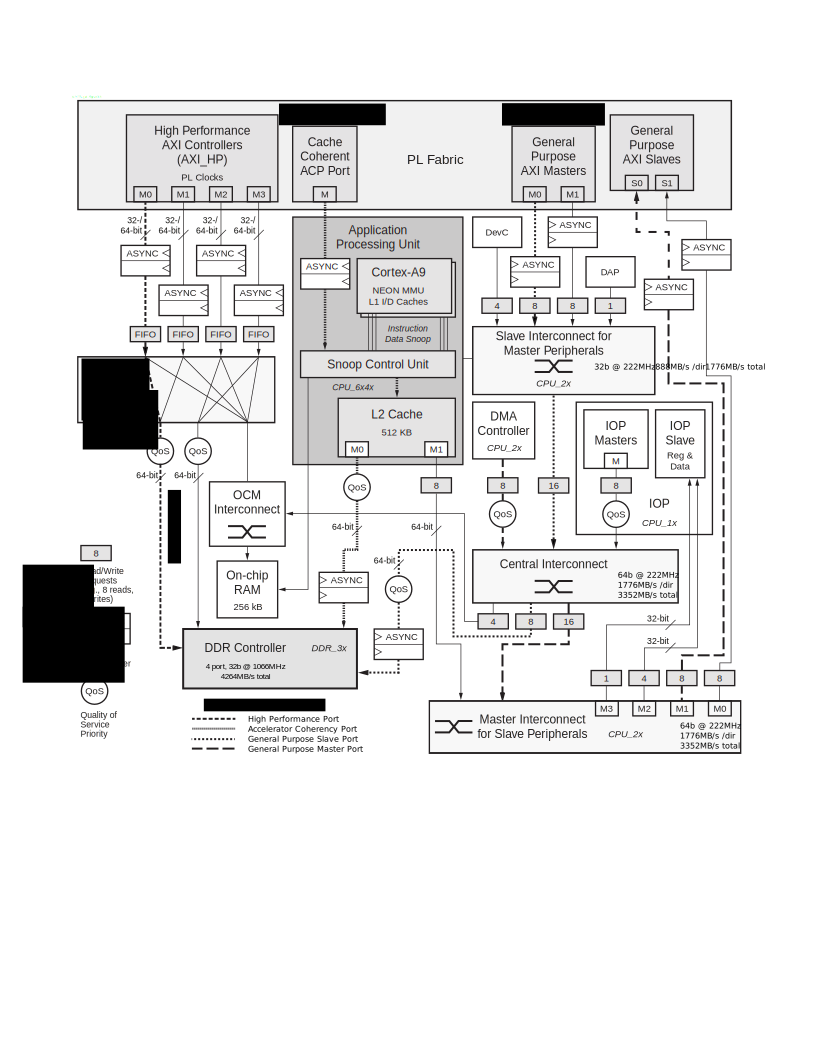
\includegraphics[scale=.9,center,trim={0 75mm 0 0},clip]{img/zynq-7000.pdf}
  \caption{The Zynq 7000 system architecture. 
  Note that port naming follows the controller role, not the port's.
  For example, the ``GP \gls{axi} Masters'' are connected to the
  ``GP \gls{axi} Slave Ports'', titled ``M0'' and ``M1''. Conversely,
  the ``GP \gls{axi} Slaves'' are connected to the ``GP \gls{axi} Master Ports'', titled ``S0'' and ``S1''.
  Modified image from \cite{ug585}.
  }
  \label{fig:zynq7000-interconnect}
\end{figure}

\subsubsection{The High Performance Ports}

The Zynq 7000 provides four \gls{hp} ports, HP0 to HP3.
These are all \gls{axi} slave ports to the PL,
connecting a Full \gls{axi}3 master at the PL endpoint. 
If the \gls{axi} master is implemented in \gls{axi}4, as is the usual case,
a protocol conversion must take place before connection.

The ports are clocked by a PL clock, at up to 150MHz, and can be 32 or 64 bit wide.
As the \gls{axi} protocol mandates, they have separate wires for each direction,
offering a per direction bandwidth of 1200MB/s for each port.

The \gls{hp} ports are connected to the memory controller through the Memory Interconnect
which in turn drives two of the four ports of the memory controllers, as well as
one port of the \gls{ocm} interconnect.
The port clock will be converted to 355MHz,
offering a switching speed of 2840MB/s per direction, 5680MB/s total.
The switching scheme routes the traffic from the first two \gls{hp} ports 
to the first memory port, and the other two \gls{hp} ports to the second. 

The memory controller offers an aggregate bandwidth of 4264MB/s 
shared among its four ports, irrespectively of the data flow direction.
Therefore, if all \gls{hp} ports are used and configured at their maximum ratings,
the maximum theoretical bandwidth of 9600MB/s will be first saturated by the
memory interconnect, and if the OCM path is not used, will be further constricted
by the memory controller.

\subsubsection{The Accelerator Coherency Port}

The ACP port, compared to the \gls{hp} ports, 
has equivalent performance specifications.
The connectivity to the memory subsystem, 
however, is totally different.
As it was mentioned in \ref{amba}, 
the ACP port needs to be in close proximity to the
processor in order to provide cache coherency 
to traffic generated from a non-coherent \gls{axi} master.
Indeed, in Zynq-7000 series the \gls{acp} port is connected 
directly to the Snoop Control Unit of the L2 Cache. 
From there, it can access one dedicated 
port of the memory controller.
This is a low latency path to memory, 
but its tight relationship with the processor
will complicate the usage scenarios.

\subsubsection{The General Purpose Slave Ports}
\label{sect:sgp}

The GP slave ports offer the half of the data width 
of the \gls{hp} ports as they are 32 bit only,
but they can operate at up to the same frequency of 150MHz. 
Nonetheless, in order to reach the memory controller 
they follow a much more complicated path.

Firstly they reach the Slave Interconnect. 
They occupy two of its four slave ports,
the other being dedicated to the 
\gls{devc} controller and the \gls{dap}.
Note that the former will be heavily used as it is responsible
for programming the FPGA during partial reconfiguration.
The Slave Interconnect operates at 222MHz, 
offering an aggregate bandwidth of 888MB/s per direction.

The master port of Slave Interconnect is connected to
Central Interconnect, which operates also at 222MHz but
has a width of 64 bits, totalling at 1776MB/s per direction.

The Central Interconnect is shared by another two masters:
The PS DMA controller and the I/O Peripherals
(the flash memory interfaces, the USB and Ethernet controllers, etc).
Itself is master to three peripherals:
The OCM interconnect to leads to \gls{ocm} memory, the Master Interconnect
which connects the PL masters to the \gls{fabric} via the \gls{mgp} ports,
and finally, one port of the memory controller.

It is obvious that in order for \gls{sgp} to reach the memory controller,
it has to cross two rather busy interconnects and resource competing
could become an issue.

\subsubsection{The General Purpose Master Ports}

The GP master ports are the funcional opposite of GP slave ports;
they can connect PL slaves and they route the traffic through the
Master Interconnect which in turn is a slave to the Central Interconnect.
It is important to note that they are the only master ports from the PS side.
If any transaction has to be started with the initiative of the PS,
it \emph{must} pass from these ports.

\subsection{The Zynq UltraScale+ Interconnect Architecture}

The UltraScale+ series has significantly improved the system interconnect.
Apart from the expected increase in number and bandwidth of the
PS-PL ports and their pathway to the memory, there is much better support
for cache-coherent peripherals. 
Unlike the 7000 series, in UltraScale+ 
all ports are of equal maximum width and frequency; 
they are all 128 bit wide and may operate at up to 333MHz.
Nonetheless, since they have different connectivity and offer different
functionality, subsequently they will also differ in access latency to
the memory controller. Additionally, they are mapped differently in the
processor address space and have varying address widths; all of them
however, are at least 32 bits.

The UltraScale+ is updated to \gls{axi}4 and therefore no protocol
conversion will happen in the PL. However, the \gls{axi} \glspl{fifo} at slave ports
are \gls{axi}3 compatible and protocol conversion will take place transparently
inside the PS domain.

An overview focused on interconnect
is displayed in figure \ref{fig:zynqmp-interconnect}. 
The reference for technical information presented here is \cite{ug1085}.

\begin{figure}[htbp]
  \centering
  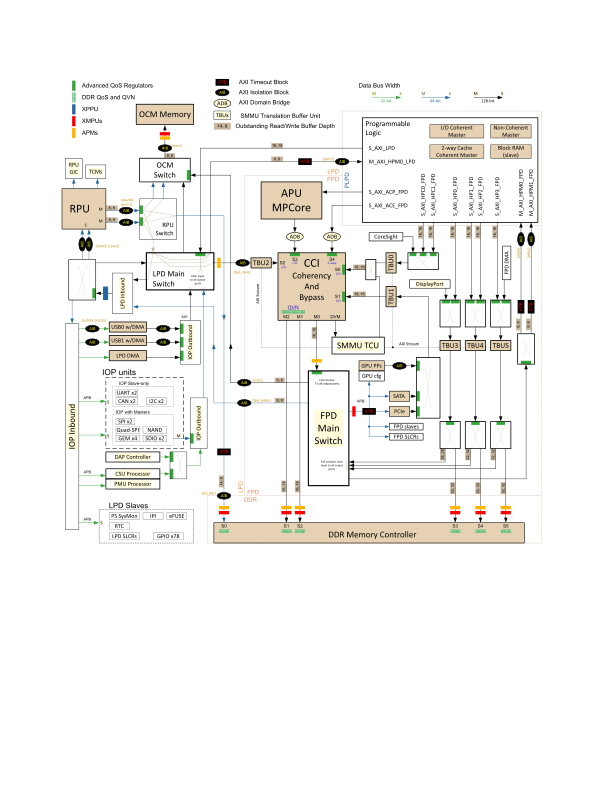
\includegraphics[scale=.9,center,trim={0 75mm 0 0},clip]{img/zynqmp.pdf}
  \caption{The Zynq UltraScale+ system architecture, image from Xilinx \cite{ug1085}.
  The naming nomenclature denotes (in order) the master or slave role, 
  the protocol (AXI), the port name with the modifier ``C'' for ``coherent'' or
  repeating ``M'' for ``master'' then followed by the port number, and finally
  the power domain designation.
  }
  \label{fig:zynqmp-interconnect}
\end{figure}


\subsubsection{High Performance Ports}
\label{sect:implementation}

The UltraScale+ features four \gls{hp} ports that reside in the \glsentrylong{fpd}.

As one can realize from figure \ref{fig:zynqmp-interconnect},
the path from an \gls{hp} port to the memory controller is not identical for all ports.
Indeed, the memory port S3 is shared between HP0 and DisplayPort controller
while the S5 is shared between HP3 and the \gls{fpd} DMA.
The interfaces HP1 and HP2 share exclusive access to memory port S4,
a property to be considered if the lowest latency 
or a deterministic performance is desired. Additionally, if the DisplayPort
controller is not used, the HP0 will have full bandwidth access to the S3 memory port.
The HP3 would be the least attractive to use, 
since the access pattern of the \gls{fpd} DMA may not be easy to be predicted.

\subsubsection{High Performance Coherent Ports}

As the name suggests, the \gls{hpc} ports are cache-coherent versions of \gls{hp}, 
albeit \glslink{IO Coherency}{IO coherent} only, much like the \gls{acp} port. 
However, in contrast to the \gls{acp},
the coherency is not ensured by the \gls{scu} but by the \gls{cci}.

Decoupling the port from the processor has both its benefits and its shortcomings. 
The \gls{hpc} ports have higher latency than \gls{acp} to the memory controller,
even higher than \gls{hp} ports since they have to cross \gls{cci}.
On the other hand, it does not share a path with the processor to the cache,
alleviating the resource competing in a such an important pathway.
Xilinx labels the \gls{acp} as a ``legacy'' port, 
showing its preference in \gls{hpc}.

There are two such ports in UltraScale+. They share access to a single
port of the \gls{cci}, which they can reach after crossing two switches.
From there, they can be routed to the two memory ports that are visible
to the \gls{cci}.

\subsubsection{High Performance Master Ports}

Essentially, the \gls{hpm} ports inherit the role of Zynq-7000's \gls{mgp} ports.
They are masters to the PL, so they are the gateway for any traffic generated with
the initiative of the PS, that being the ARM cores or the PS DMA controllers.

There are three such ports. Two of them are in the \gls{fpd} and one in the \gls{lpd}.
Unlike Zynq-7000, their performance is not inferior to \gls{hp} ports.

\subsubsection{The AXI Slave Port of LPD}

There is a single slave AXI port that connects the PL to the \acrlong{lpd}.
The port is connected to the LPD Main Switch, and from there is routed to the \gls{rpu}
after crossing two further switches. 
Along with the \gls{lpd} \gls{hpm}, 
they are the only means of accessing the PL from
\gls{rpu} side without crossing the \acrlong{fpd}.


\subsubsection{Accelerator Coherency Port}

Retained albeit unfavored from the Zynq-7000 series, the \gls{acp} port
is upgraded to match the performance of the other UltraScale+ ports.
Only one such a port is available.

\subsubsection{AXI Coherency Extensions Port}

The \gls{ace} port is a unique addition to this FPGA-SoC family. 
With the help of \gls{cci} it can offer two-way, full cache coherency.
That is, it can support a cache-enabled peripheral and maintain coherency of both
the processor's and the peripheral's cache.

\section{Exchanging Data with the Programmable Logic}

The diversity of the physical interconnect creates a number of 
possible methods for transferring data between PS and PL.
Each method may benefit a specific transfer pattern
or may be more appropriate for an application.
The temporal characteristics of the transfer,
the amount of data to be transmitted, 
tha requirements for latency or thoughput,
the power consumption and the need of a higer level of determinism,
all of them will define the optimal solution for each problem.

Let us now discuss the possible scenarios.

\subsection{Programmed I/O from a Processor}

The Zynq 7000 features two ARM Cortex-A9 processor cores
that can generate load/store requests. These may target
the DDR memory and the \gls{ocm} directly from the cache ports
and the \gls{scu} respectively, or the PL through the means
of Master Interconnect (see \ref{fig:zynq7000-interconnect}).1

The UltraScale+ is a bit more complicated since it features
two processor clusters that use different pathways.
The high-power A53 cores in \gls{apu} are connected to the \gls{cci}
and from there they may reach either the DDR memory controller,
or be routed from FPD Main Switch either to one of the \acrlong{hpm}s to reach the PL,
or the OCM Switch to reach the \gls{ocm}.
The low-power R5 in \gls{rpu} can only send to the RPU Switch.
From there it can reach three targets: 
The OCM Switch that provides access to the \gls{ocm},
the DDR memory controller directly,
and the \gls{lpd} \gls{hpm} that gives access to the PL.
Additionally, it has a link to the \gls{cci} through the LPD Main Switch
from where it can be routed anywhere in the \acrlong{fpd}, including the \gls{fpd} \glspl{hpm}.

Overall, the main advantage should already be obvious:
The Programmed I/O method can low-latency access to any component of the PS and the PL,
without the need of any PS or PL third-party actor, like a DMA controller. Thus, it saves
resources on both PS and PL.

The second big advantage is simplicity. From software point of view, 
it is sufficient that the program issues the appropriate load / store instructions,
with a possible memory barrier -- no initialization of any component.
As for hardware, an slave peripheral is sufficient to
implement an \gls{axilite} interface, which is low demanding in complexity and resources.

The major drawback derives from the very nature of programmed I/O and is not Zynq specific.
The fact that the traffic is generated by load / store instructions is a twofold problem:
First it keeps the processor busy issuing the instructions preventing it 
to perform any other useful work. The problem aggravates as the number of slaves increases,
as obviously there cannot be more parallel transfers than the number of processors executing I/O.
Secondly, the load / store instructions cannot generate \gls{burst} transfers,
essentially degerating a full \gls{axi} to \gls{axilite}. 
According to Xilinx (\cite{ug585}, v1.11, pg. 656) one should expect 
transfer rates of around 25MB/s in Zynq-7000.

The most common use case for this method is writing configuration registers,
reading status or other initialization work. 
Such small data exchanges are latency sensitive, not throughput,
making a perfect fit for programmed I/O.

\subsection{Using the PS DMA}

The Zynq-7000 features an eight-channel DMA controller on the PS side.
Looking back at figure \ref{fig:zynq7000-interconnect} we can see that it is connected
with a single link to the Central Interconnect. 
From there, it may reach the DDR Controller directly, the \gls{ocm} memory through the
OCM Interconnect, and finally, through the Master Interconnect, it may reach the PL by
using one of the \glspl{mgp} (the coarsely dashed line). 

The UltraScale+ has two DMA controllers, one in the \glsentrylong{fpd} and one
ine the \glsentrylong{lpd}. 
The \gls{fpd} DMA controller shares a link with the \gls{hp}3. The link
is driven to a second switch that gives access to either the DDR memory controller,
or it is routed to the FPD Main Switch, in turn to the OCM Switch, and finally the \gls{ocm}.
The \gls{lpd} DMA controller is connected to the I/O Peripheral Outbound Switch that is
connected to the LPD Main Switch. From there it can see the OCM Switch and the \gls{ocm} memory,
the DDR memory controller, or it can enter the PL via the LPD \gls{hpm}.

The DMA controllers can be programmed by a PS processor. The programming of a DMA controller
is certainly a more complex matter than just issuing a load / store instruction,
so an increase of software complexity is for granted. 
However, the obvious advantage is that they come ``for free'', that is,
they are already present in the silicon, not consuming any PL resources.
They are multi-channel and they can provide a throughput of at least an order
of magnitude higher than programmed I/O, without keeping busy the processor.

However, as we saw, the flow of data crosses a lot of already busy interconnects.
The sharing of bandwidth reduces all aspects of performance, 
including its predictability and repeatability -- of all users.
We shall not forget also, that even the DMA controllers are actually shared with
other system components, eg the network driver will typically use it to transfer data
to/from the network interface. On top of that, the master ports in both 7000 and UltraScale+
are fewer, and in the former, are also narrower.

Specifically for this work, it should be added that PS DMA is full \gls{axi} compatible
and has no \gls{axistream} -- and neither of the ports of 7000 or UltraScale+ are 
\gls{axistream}-compatible anyway. That means that once the traffic is in the PL,
it must be converted to \gls{axistream}. 
The PL resources needed for this conversion are comparable to implementing a DMA
controller directly to the PL, making this choice appear unattractive.

All in all, the use of the PS DMAs is a viable solution, 
albeit certainly not the best performant. 
To make things worse, it does not map favorably to the goals of this work.
Therefore, this solution was abandoned.

\subsection{Implementing a DMA controller in the PL}

Modern FPGAs are large enough to allow us 
the possibility to implement our own DMA controllers 
at a tolerable cost in PL resources. 

The sacrifice of PL resources is not trivial.
However this drawback could be offset by the number of
advantages that this method gives us:

\begin{itemize}
\item	Both Zynq series feature significantly more 
	slave ports to the PL than master ones.
	Their parallel use would increase aggregate bandwidth.
\item	There is the oportunity to use other interconnect pathways that are not
	being used by the usual client peripherals, alleviating the potential
	issue of an interconnect bottleneck.
\item	Using a path that does not cross the Central Interconnect and the
	Master or Slave Interconnect would have the benefit of 
	reduced and more predictable latency. 
	In the extereme case, one could dedicate a whole pathway 
	for a specific latency critical accelerator.
\item	The PS DMA would be freed for use by other services, 
	especially the network driver.
\item	We gain the flexibility implement the PL DMA
	exactly according to our specific needs.
	It could itself become grounds for research,
	as the capability of the DMA controller
	plays a significant role in overall system performance.
\item	It opens the possibility for the design of more complicated 
	architectures than our case of an isolated accelerator 
	that reads from memory, processes, and writes back.
	For example, output could be re-routed to 
	another accelerator or to an external device
	(ie chip to chip data exchange, data aquisition or data display)
	without the need of going back and forth to the main memory.
\end{itemize}

The choice of slave port however, is a decisive factor 
as it can deny us several of the aforementioned advantages.
Therefore, they should be treated separately.

\subsubsection{The HP ports}

In Zynq-7000 series, the \gls{hp} ports have an 
exclusive access to two memory ports 
through the memory interconnect.
This is an impressive feature, considering that the processor and
the Central Interconnect have only one each.
Furthermore, by having four of them, 
we gain significant flexibility on the AXI interconnect
that it will need to be implemented at the PL side.

Similarily, in UltraScale+, the four \gls{hp} ports have
access to three memory ports, after crossing two rows of switches.

The primary drawback of these ports is that they are not cache-coherent.
In this implementation, the access pattern is a continuous stream of data
that flow through the accelerator. That pattern has zero temporal locality --
caching the data would be useless if not harmful.

Therefore, these ports would be the prime candidates for connecting 
the accelerators.

\subsubsection{The HPC ports (UltraScale+ only)}

The \gls{hpc} ports, in contrast to \gls{hp}, cross the \gls{cci} to reach
the memory controller. This has two side effects: Firstly, they can 
optionally be cache-coherent, and secondly, the crossing of \gls{cci}
will induce a latency penalty.

Eventually, since cache coherency is not important for this implementation,
the \gls{hp} ports will be preferred. However, despite that \gls{hpc} ports
incure a small latency, they offer a path to access two further memory controller
ports, increasing our potential bandwidth by 66\%. 
Therefore, they will be used in addition to the \gls{hp} ports, albeit with
cache coherency disabled.

\subsubsection{The ACP port}

The \gls{acp} port is an interesting addition not only due to its \glslink{IO Coherency}{IO coherent}
nature, but also due to its proximity with the processor. 
The \gls{acp} port would be ideal in an access pattern where the processor and the PL accelerator
work together, exchanging small pieces of data or cooperatively working in the same dataset.
Essentially, the ``accelerator'' would be more of a ``coprocessor''.
In this access pattern, the data generated from the processor would stay in cache, from where
the \gls{acp}-connected accelerator will retrieve it, without accessing the DDR memory at all.
This would have a huge benefit to memory throughput and
would alleviate the traffic of the memory controller. Additionally, since retrieving data
from cache is an order of magnitude cheaper in energy than retrieving from memory,
the power efficiency of the system would dramatically improve.

Nonetheless, this is not our case. Our streaming data pattern would 
cause continuous cache misses and cache thrashing,
increasing the latency and depriving the processor any cached memory.
Furthermore, the \gls{acp} and the processor core share the connectivity
of the \gls{scu} to the L2 cache, competing for access.
Performance-wise it would be a disaster and therefore it will not be attempted.

\subsubsection{The ACE port}

The ACE protocol differs from both \gls{hpc} and \gls{acp} 
in that it offers full, two-way coherency. This permits
maintaining cache coherency between the processor with caches and a
full \gls{axi} peripheral with cache in the form of \gls{bram}.

In comparison to \gls{acp}, the \gls{ace} (and also the \gls{hpc}) do not compete
with the processor for cache access. 
Yet, the \gls{ace} adds significant complexity to the slave and the interconnect.
Its access to the memory controller is through the \gls{cci}, an access already
gained through \glspl{hpc}, leaving us little incentive to use this port.

\subsubsection{The S\_GP in 7000 and the LPD Slave AXI in UltraScale+}

In section \ref{sect:sgp} it was described how \gls{sgp} can reach the memory controller.
It is a complex path that comprises crossing both the Slave Interconnect and the Central
Interconnect. That cancels out a couple of our initial arguments for the use of the slave ports.
Further discouraging is the fact that we will compete 
with the \gls{devc} which controls the single \gls{pcap}
port thay may reconfigure the FPGA.

Still, the \gls{sgp} will open us access to one more port to the DDR controller.
For this very reason, it is worth to experiment using it.

The LPD Slave AXI port of the UltraScale+ shares some characteristics with \gls{sgp}.
However, studying the figure \ref{fig:zynqmp-interconnect} we will see that the port
can reach the memory controller through the LPD Main Switch and the \gls{cci},
not the RPU Switch, whose only master is the \gls{rpu} itself.
This actually the case even for the LPD DMA.

This was an intended design decision. The \gls{rpu} needs exclusive access to the
memory controller in order to offer predictable and repeatable access latency,
a key characteristic of its real-time nature.

Therefore, there is not much incentive to use it, since we already access the
memory ports of the \gls{cci} via the \glspl{hpc}.

\section{Implementing the Interconnect}


\subsection{Configuring the DMA}

In order to quantify the use of resources a test design was used to
measure the resource usage of the AXI DMA IP core.

\begin{figure}[ht!]
\centering
\begin{tabular}{cl rrrrr rrrrr}
\toprule
	&\multicolumn{5}{r}{32 bit data} & \multicolumn{5}{c}{64 bit data}\\
&		& DR 	& SG 	&\multicolumn{3}{c}{SG+MC}& DR 	& SG 	&\multicolumn{3}{c}{SG+MC}\\
&		&	&	& 1ch	& 8ch	& 16 ch	&	&	& 1ch	& 8ch	& 16	\\
\midrule
\multirow{5}{*}{\rotatebox[origin=lB]{90}{7000}}
&LUT		& 1571	& 2076	& 2696	& 3245	& 3877 	& 1811	&	&	&	&	\\
&FF		& 1996	& 3235	& 3807	& 4188	& 4626	& 2394	&	&	&	&	\\
&BRAM36		& 2	& 2	& 2	& 2	& 2	& 2	&	&	&	&	\\
&BRAM18		& 0	& 0	& 0	& 0	& 0	& 2	&	&	&	&	\\
&Nets		& 404	& 593	& 637	& 637	& 637	& 544	&	&	&	&	\\
\midrule
\multirow{5}{*}{\rotatebox[origin=lB]{90}{UltraScale+}}
&LUT		& 	& 	& 	&	& 	& 	&	&	&	&	\\
&FF		& 	& 	& 	&	&	& 	&	&	&	&	\\
&BRAM36		& 	& 	& 	&	&	& 	&	&	&	&	\\
&BRAM18		& 	& 	& 	& 	&	& 	&	&	&	&	\\
&Nets		& 	& 	& 	&	&	&	&	&	&	&	\\
\bottomrule
\end{tabular}
\caption{Resource usage of the AXI DMA core. Configured with burst size 16, address width 32 bits\\
	LUT: Look-up tables, FF: Flip-flops, BRAM36/18: Block RAM 36kb/18kb, Nets: Boundary Nets\\
	DR: Direct Register, SG: Scatter-Gather, MC: Multi-channel, $n$-ch: number of channels}
\end{figure}

\begin{figure}[ht!]
\centering
\begin{tabular}{cl c ccccc c ccccc}
\toprule
	&	&& \multicolumn{4}{c}{Zynq 7000}	&& \multicolumn{4}{c}{Zynq UltraScale+}\\
	&	&~~~& LUT	& FF	& BRAM 	& Nets	&~~~& LUT	& FF	& BRAM	& Nets \\
\midrule
\multirow{5}{*}{\rotatebox{90}{32 bit data}}
	& DR	&& 1571	& 1996	& 2/0	& 404	&&	&	&	&	\\
	& SG	&& 2076	& 3235	& 2/0	& 593	&&	&	&	&	\\
	& MC 1ch	&& 2696	& 3807	& 2/0	& 637	&&	&	&	&	\\
	& MC 8ch	&& 3245	& 4188	& 2/0	& 637	&&	&	&	&	\\
	& MC 16ch	&& 3877	& 4626	& 2/0	& 637	&&	&	&	&	\\
\midrule
\multirow{5}{*}{\rotatebox{90}{64 bit data}}
	& DR	&& 1811	& 2394	& 2/2	& 544	&&	&	&	&	\\
	& SG	&& 2362	& 3636	& 2/2	& 733	&&	&	&	&	\\
	& MC 1ch	&& 2978	& 4208	& 2/2	& 777	&&	&	&	&	\\
	& MC 8ch	&& 3527	& 4589	& 2/2	& 777	&&	&	&	&	\\
	& MC 16ch	&& 4159	& 5027	& 2/2	& 777	&&	&	&	&	\\
\bottomrule
\end{tabular}
\caption{Resource usage of the AXI DMA core. Configured with burst size 16, address width 32 bits\\
	LUT: Look-up tables, FF: Flip-flops, BRAM: Block RAM (36kb/18kb), Nets: Boundary Nets\\
	DR: Direct Register, SG: Scatter-Gather, MC: Multi-channel, $n$-ch: number of channels}
\end{figure}


